\chapter{Software Engineering Process}\label{sec:agile}

This chapter discusses the software engineering process that was followed to design and build the codeHelper system.

Developing software in an entirely plan-driven way, where the requirements are specified completely before and the design, building and testing follow, is not a development process which gives rapid software development \cite{sommerville}. 

Given that the outline of this project was for a novel system, it was likely that requirements would change and problems would be discovered during development. In an exclusively plan-driven approach to engineering, this would result in the system design or implementation having to be reworked and retested (shown in figure \ref{fig:planspec}) - increasing the timescale of the project \cite{sommerville}.

\begin{figure}[H]
    \centering
    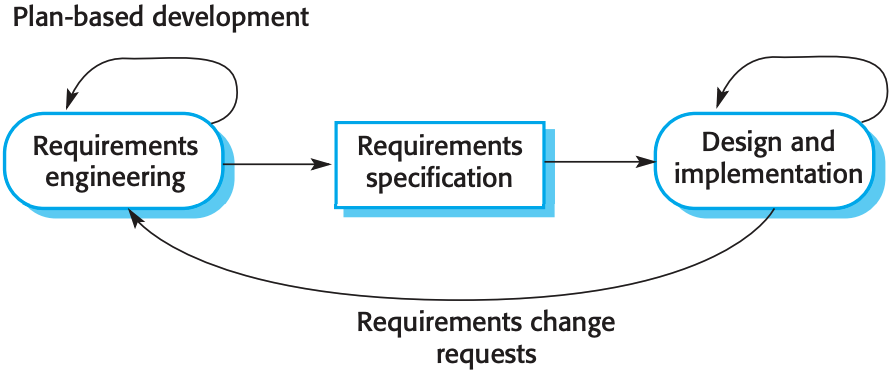
\includegraphics[width=0.6\textwidth]{6swengprocess/images/planspec.png}
    \caption{The plan-driven approach to system specification \cite{sommerville}.}
    \label{fig:planspec}
\end{figure}

As a result, the methodology chosen for development of the system was agile software development. 


\begin{figure}[H]
    \centering
    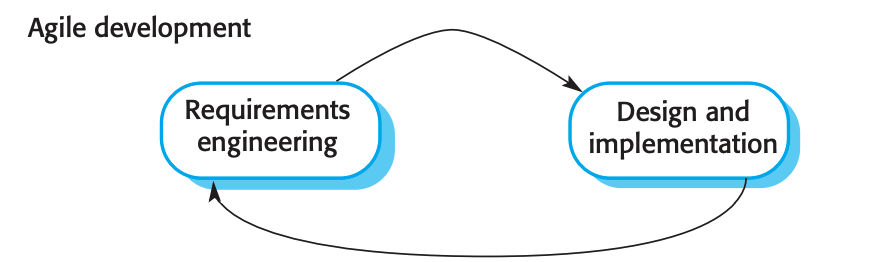
\includegraphics[width=0.6\textwidth]{6swengprocess/images/agilespec.png}
    \caption{The agile approach to system specification \cite{sommerville}.}
    \label{fig:agilespec}
\end{figure}

Agile software development is an approach which is incremental, cooperative (customer and developers working constantly together with close communication), straightforward (the method itself is easy to learn and to modify), and adaptive (able to make last moment changes) \cite{Abrahamsson}. 

The fact that increments are small and, typically, new iterations of the system are made every two or three weeks \cite{sommerville} as well as the fact that customer (supervisor) involvement is frequent throughout the process make an agile approach ideal for the project. Given the timescale, rapid feedback was critical to successful development of the codeHelper application. Figure \ref{fig:agilespec} shows the approach to system specification in agile methods and should be compared to figure \ref{fig:planspec}.

In practice, a methodology close to Scrum was followed throughout the project. 

To begin the project, there was an initial planning phase as outlined by Scrum and required by the nature of a Master's dissertation. During this phase, the architecture of the project was defined. However, during development, adjustments were made to this architecture as outlined by Scrum \cite{scrum}. During the planning phase, Trello \cite{trello} was used to store a list of currently identified tasks (see Figure \ref{fig:backlog}), known in Scrum as a backlog \cite{scrum}.

\begin{figure}[H]
    \centering
    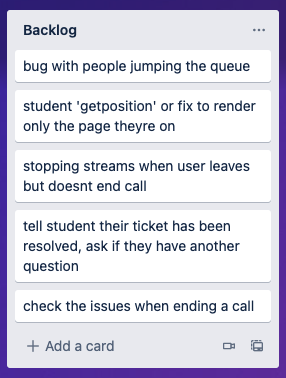
\includegraphics[width=0.4\textwidth]{6swengprocess/images/trelloBacklog.png}
    \caption{Example of scrum backlog of tasks on Trello during the project.}
    \label{fig:backlog}
\end{figure}

After minimal initial planning, Scrum purports a series of short development phases, or sprints (see Figure \ref{fig:scrum}), deliver the product incrementally \cite{scrum}. Sprints aim to produce a visible, usable product that implements one or more user interactions with the system - to deliver valuable functionality \cite{scrum}. These sprints were one week long, since the supervisor meetings were weekly. At the beginning of each sprint, tasks in the backlog were updated and prioritised before identifying the tasks that should be completed in that sprint. Tasks in the project were designed to be specific enough to be completed in a week or less (see Figure \ref{fig:backlog}). 

\begin{figure}[H]
    \centering
    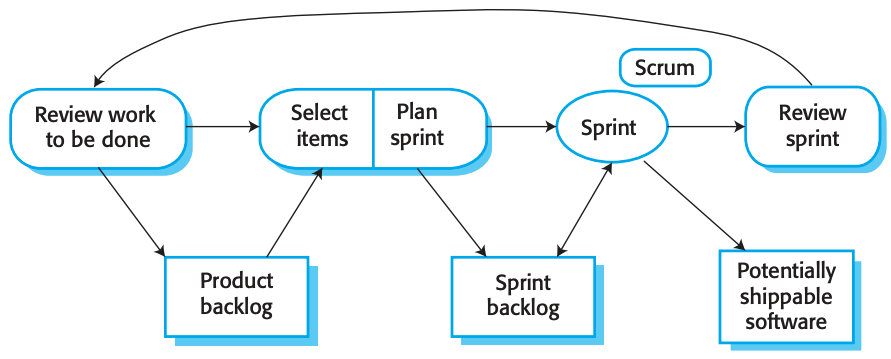
\includegraphics[width=0.65\textwidth]{6swengprocess/images/scrum.png}
    \caption{The scrum sprint cycle \cite{sommerville}.}
    \label{fig:scrum}
\end{figure}

Weekly supervisor meeting offered the chance to review each sprint, since the project supervisor is also the product owner or customer. During these meetings, project goals and tasks can be added, eliminated or reprioritised. In this project as in application of Scrum in industry, items which the customer prioritises must have the highest development priority \cite{scrum}.